\subsection{Performance Requirements}
\begin{itemize}
	
\end{itemize}
\subsection{Design Constraints}
\begin{enumerate}
	
\end{enumerate}
\subsection{Software System Attributes}



\subsection{Class diagram}
 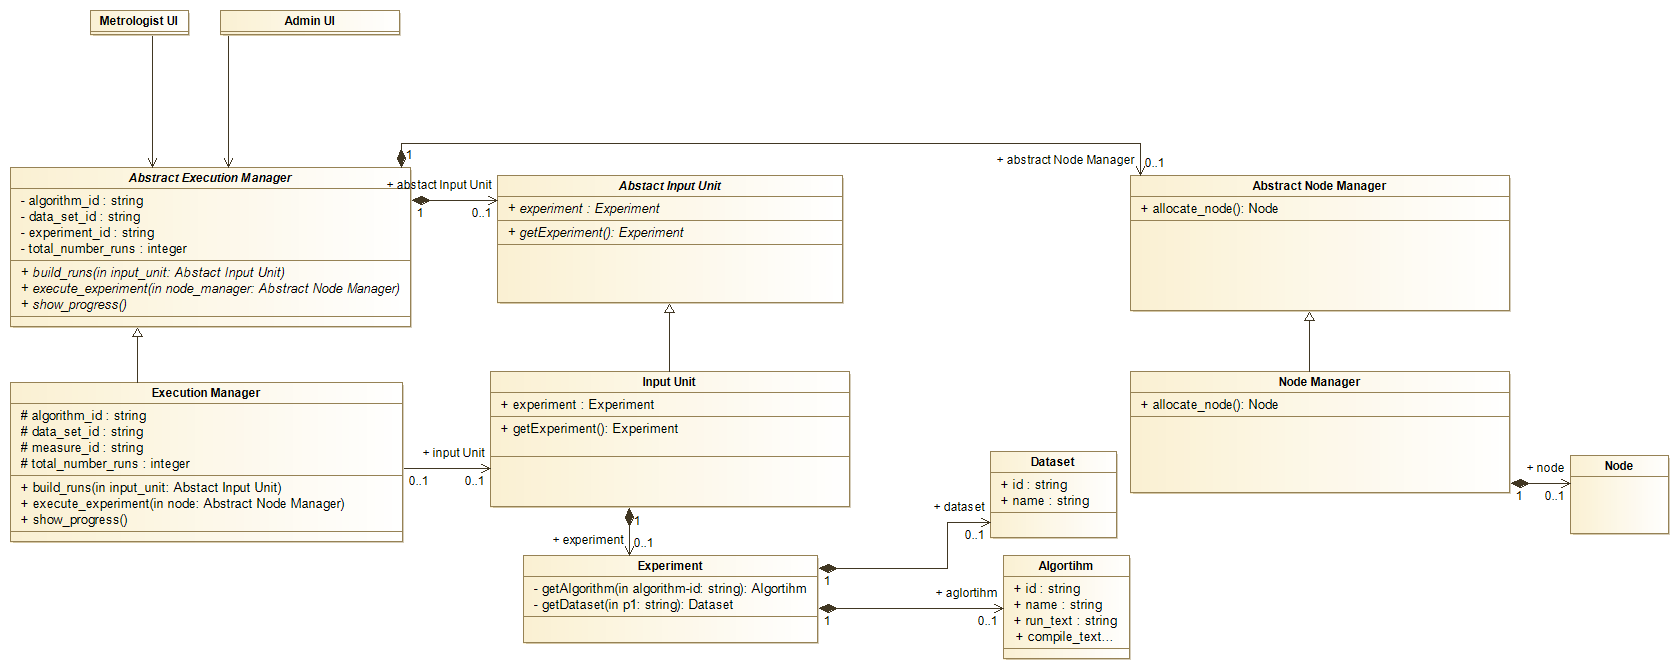
\includegraphics[width=\textwidth]{admin_ui/images/execution_manager_class_diagram.png}
	\begin{center}
	    \small{Figure #: Class diagram for Execution Manager}
    \end{center}
    
    \paragraph{\textbf{Design Pattern Used} \\ \\
	I used the mediator design pattern because the execution manager uses the input unit as well as the node manager to perform the build runs and execute experiment respectively. The execution manager also persists to the admin UI and the Metrologist UI thus a pattern that can communicate with the reinvent modules and not be extremely dependent is needed. That is why I selected the mediator pattern because it encapsulates the way that objects communicate with each other thus the relevant modules can communicate with each other without knowing the components underlying structure. By using this pattern the modules will be loosely coupled which makes the overall structure of the system much better and easier to manage.In this case the mediator is the \textbf{Execution Manager}  is the Mediator. The \textbf{Input Unit} and \textbf{Node Manager } are the colleagues of the mediator. The \textbf{Metrologist} and \textbf{Admin UI} are the colleagues and as you can see modules are encapsulated.}
		
\subsection{Activity diagram}
    %\includegraphics[width=\textwidth]{}
	\begin{center}
	    \small{Figure #: Activity diagram for ...}
    \end{center}


\subsection{Sequence diagram}
    %\includegraphics[width=\textwidth]{}
	\begin{center}
	    \small{Figure #: Sequence diagram for ...}
    \end{center}

\subsection{State diagram}
    %\includegraphics[width=\textwidth]{}
	\begin{center}
	    \small{Figure #: State diagram for ...}
    \end{center}




\subsection{Use Case diagram}
    %\includegraphics[width=\textwidth]{}
    \begin{center}
    	\small{Figure #: Use case diagram for ...}
    \end{center}